\chapter{Perifer interaktion}
\label{PeriferInteratkion}
%
Skriv en hat for hele kapitlet
%
\begin{itemize}
  \item Socialt acceptabelt 
\end{itemize}
\noindent
%
Perifer interaktion er ikke nyt. Vi gør det alle sammen, når vi i løbet af vores dagligdag foretager adskillige aktiviteter i vores perifere opmærksomhed, \parencite[s. 1]{PDF:PeripheralInteraction}. Det forudsætter dog at disse perifere interaktioner primært retter sig mod ikke-computer-relateret aktiviteter, såsom at føre en samtale imedens der laves mad. Rettes fokus derimod til \textit{Human-Computer-Interaction}, HCI, så forlanger diverse elektroniske apparater vores centrale opmærksomhed ved at blinke, ringe og vibrere, \parencite[s. 1]{PDF:PeripheralInteraction}. Ifølge \textcite[s. 3]{PDF:PeripheralInteraction} så bevæger interaktionen med elektroniske apparater sig uforudsigeligt mellem den centrale og perifere opmærksomhed, i modsætning til ikke-computer-relateret aktiviteter, som i større grad kan kontrolleres. Grunden til at disse apparater frit kan bevæge sig fra den perifere til den centrale opmærksomhed skyldes, at vi sjælendt har kontrol over hvornår et apparat kræver den centrale opmærksomhed. Så snart et elektronisk apparat befinder sig i den centrale opmærksomhed, så vil ens opmærksomhed midlertidigt fjernes fra den primære opgave, indtil interaktionen med apparatet er afsluttet. Konsekvenserne af at blive forstyrret og skulle rette opmærksomheden væk fra ens primære opgave over til apparatet, er en øget kognitiv belastning samt en større risiko for at begå fejl i den primære opgave, \parencite[ss. 188-189][s. 162]{PDF:PeripheralInteraction, PDF:ComparingInputModalities}. 

Istedet for at forstætte med at designe elektroniske apparater, som både kræver den centrale opmærksomhed og kræver at opmærksomheden flyttes væk fra den primære opgave, så bør apparaterne derimod designes så de i højere grad bliver en integreret del af vores daglige rutiner, \parencite[s. 239]{PDF:PICharacteristicsAndConsiderations}. Ved at designe apparater ud fra den tilgang så vil det tillade perifer interaktion, fordi det, blandt andet, bygger på teori omkring delt-opmærksomhed. Ifølge disse teorier råder mennesket over en bestemt mængde af mentale resourcer, som afhængigt af opgavernes sværhedsgrad, frit kan distribueres mellem opgaverne, \parencite[s. 240]{PDF:PICharacteristicsAndConsiderations}. Derudover tillader delt-opmærksomhed også at flere aktiviteter kan foretages samtidigt, så længe de kun kræver få mentale ressourcer, \parencite[s. 2]{PDF:FacilitatingPIDesignAndEvaluation}. Så istedet for at elektroniske apparater kræver den fulde opmærksomhed, så er det ved perifer interaktion muligt at distribuere sin opmærksomhed for på den måde at foretage flere aktiviter samtidig. Hvis interaktion med computere og andre elektroniske apparater blev flyttet til det perifere kan det, ifølge \textcite[s. 11]{PDF:TheComputerWeiser}, potentielt være med til at fremme det sociale samvær, som der eksempelvist er på arbejdsmarkedet. Derudover pointerer \textcite[s. 11]{PDF:TheComputerWeiser} at de elektroniske apparater skal tilpasses til den menneskelige hverdag og ikke omvendt. Ligeledes bør der tages højde for at desto flere elektroniske apparater, der produceres til at fange vores centrale opmærksomhed, desto større er behovet for at en del af interaktionen bliver perifer, \parencite[s. 240]{PDF:PICharacteristicsAndConsiderations}. \blankline
%
Behovet for at designe elektroniske apparater, som tillader perifer interaktion er ikke nyt. Allerede i halvfemserne blev der af \textcite[s. 3]{PDF:TheComingAgeOfCalmTech} efterspurgt, at såfremt apparaterne skulle være allevegne, så skal de ikke være i vejen. I den forbindelse blev \textit{Calm Technology} skabt. Principperne bag \textit{calm cechnology} er simple; ved at allokere noget af interaktionen til det perifere er det muligt, at håndtere flere informationer ad gangen. Derudover vil denne allokering give en følelse af kontrol, fordi det er muligt selv at kontrollere hvornår noget er i den centrale kontra den perifere opmærksomhed, \parencite[s. 4]{PDF:TheComingAgeOfCalmTech}. Udover perifer interaktion, som blandt andet bygger på \textit{calm technology}, tyder det på, at der også kan drages nytte af \textit{Casual Interaction}. Ifølge \textcite[ss. 118-119]{PDF:PeripheralInteraction} vedrører \textit{casual interaction} hvor meget kontrol, der overdrages til et elektronisk apparat. Med \textit{casual interaction} er det muligt at designe apparater, som kan interageres med over en større afstand, som kræver færre kognitive resourcer, som kan interageres med ved hjælp af andre objektet og som kan interageres med uden stor præcision, \parencite[s. 128]{PDF:PeripheralInteraction}        
%
\begin{figure}[H]
	\centering
	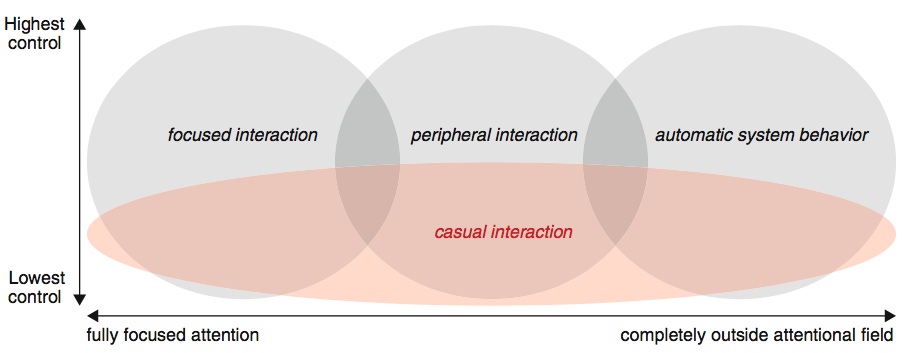
\includegraphics[resolution=300,width=\textwidth]{LevelsOfInteraction}
	\caption{Sammenhæng mellem de tre niveauer af interaktion; fokuseret, perifert og automatisk og hvilket niveau af kontrol, der ønskes samt mængden af opmærksomhed,  \parencite[s. 118]{PDF:PeripheralInteraction}.}
	\label{fig:LevelsOfInteraction}
\end{figure}
\noindent
%
Ved alle tre interaktionsniveauer er det muligt at overdrage kontrol til et elektronisk apparat, hvormed interaktionen bliver afslappet, jævnfør \autoref{fig:LevelsOfInteraction}. Det kan gøres både i den centrale, perifere og fuldautomatiske opmærksomhed. Nu hvor størstedelen af de elektroniske apparater er designet til at blive interageret med i den centrale opmærksomhed og tilmed kræver fuld kontrol, \parencite[s. 118]{PDF:PeripheralInteraction}, så må det antages, at det er det vi har vænnet os til. Men hvad så når vi står i situationer, hvor vi ikke er i stand til eller magter at have den fulde kontrol? Ifølge \textcite[s. 123]{PDF:PeripheralInteraction} kan der være tre årsager til at vi er villige til at overdrage kontrol til elektroniske apparater; 1) mentale årsager, 2) fysiske årsager og 3) sociale årsager. Et andet spørgsmål, som \textcite[s. 124]{PDF:PeripheralInteraction} stiller, vedrører om vi overhovedet er villige til at overdrage noget kontrol til de elektroniske apparater? Og svaret er, at så længe opgaven er tilstrækkeligt let og vi stadig har tilstrækkeligt kontrol til at løse opgaven, så ja, så er vi villige til at overdrage kontrol, \parencite[s. 124]{PDF:PeripheralInteraction}.\blankline
%
Udelades \textit{casual interaction} samt niveauet af kontrol, på \autoref{fig:LevelsOfInteraction}, er de resterende elementer; de tre niveauer af interaktion og mængden af opmærksomhed. Ifølge \textcite[s. 6]{PDF:PeripheralInteraction} så bliver perifer interaktion ikke udnyttet i lige så høj grad, som både fokuseret og automatisk interaktion. Til gengæld bliver der i større grad udviklet elektroniske apparater, der understøtter automatisk interaktion, som for eksempel bevægelsessensorer, der automatisk tænder lyset i et rum så snart der registreres en bevægelse, uanset om hensigten var at tænde lyset eller ej, \parencite[s. 5]{PDF:PeripheralInteraction}.\blankline
% 
Det tyder kraftigt på at der findes et stort uudnyttet område, som har et stort potentiale, hvor det er muligt at designe elektroniske apparater, som aflaster de kognitive resourcer, ikke kræver den centrale opmærksomhed, tillader tilstrækkeligt med kontrol og som potentielt kan fremme vores sociale kompetencer. Det er ihvertfald højst relevant, \parencite[s. 239]{PDF:PICharacteristicsAndConsiderations}, og nødvendigt, \parencite[s. 3]{PDF:TheComingAgeOfCalmTech}, at inddrage og udnytte mulighederne med perifer interaktion i fremtidige elektroniske apparater. 

En af udfordringerne ved at designe et elektronisk apparat, som tillader perifer interaktion er, at apparatet bør være fuldt funktionelt så det kan testes i den tiltænkte kontekst, \parencite[s. 21]{PDF:EvaluatingPI}. Det skyldes, ifølge \textcite[s. 22]{PDF:EvaluatingPI}, en kombination af at interaktionen først bliver perifer såfremt den er blevet en rutine og af at det er nødvendigt, at apparatet bliver en integreret del af ens hverdag, hvilket er vanskeligt at efterligne i et laboratorium. Så snart en interaktion er blevet en rutine, så vil det medføre at interaktionen kan udføres kun ved hjælp af få mentale ressourcer, hvilket tillader at interaktionen kan foregå i den perifere opmærksomhed, \parencite[s. 2]{PDF:FacilitatingPIDesignAndEvaluation}. Ifølge \textcite[s. 14]{PDF:PeripheralInteraction} så vil interaktionen forblive i det perifere lige indtil der opstår et problem, som ikke kan løses i det perifere, hvorfor det flyttes til den centrale opmærksomhed. \blankline 
%
Derudover bør det overvejes hvor perifer interaktion implementeres for bedst at udnytte området mellem fokuseret og automatisk interaktion. På nuværende tidspunkt tyder det på at perifer interaktion normalt egner sig til små side opgaver eller understøttende opgaver, \parencite[s. 21]{PDF:EvaluatingPI}. Hvor de små side opgaver for eksempel kan rette sig mod at ændre ens status på de sociale medier. De små side opgaver har derfor ikke en direkte forbindelse til den primære opgave, \parencite[s. 162]{PDF:ComparingInputModalities}. De understøttende opgaver retter sig mod opgaver, som har en forbindelse til den primære opgave, \parencite[s. 21]{PDF:EvaluatingPI}. Selvom de små side opgaver ikke nødvendigvis er hverken mentalt eller tidsmæssigt krævende, så vil de forårsage dels at opmærksomheden på den primære opgave fjernes og dels medføre at, der går noget tid før den primære opgave kan genoptages, \parencite[s. 162]{PDF:ComparingInputModalities}. En af årsageren til at de små side opgaver kan virke forstyrrende skyldes formegentligt at de, ligesom den primære opgave, kræver den visuelle opmærksomhed. Hvis det er tilfældet, så er det ikke muligt at udføre begge opgaver samtidig, hvorfor den ene opgave må vente til den anden er løst, hvilket referer til flaskehalseffekten, \parencite[s. 240]{PDF:PICharacteristicsAndConsiderations}. En måde at udbedre dette problem på kan, blandt andet, være at designe perifere displays, som tillader at brugeren bliver bevidst om noget information, uden det forårsager at opmærksomheden fra den primære opgave fjernes, \parencite[s. 247]{PDF:AToolkitForManaging}. Ved at allokere noget af den information, som de elektroniske apparater giver, så vil det, ifølge \textcite[s. 55]{PDF:PeripheralInteraction}, lede til en bedre brugeroplevelse i og med at brugeren ikke overbebyrdes med information, som ikke er relevant for den primære opgave. 

Det tyder på at hvis udførelsen af de små side opgaver ikke længere befinder sig i den centrale opmærksomhed, men derimod i den perifere opmærksomhed så vil det have en gavnlig effekt på den primære opgave. Ydermere tyder det på, at det kan være en fordel at overveje om interaktionen med de elektroniske apparater kan foregå helt eller delvist uden den visuelle opmærksomhed er involveret. Fokus for projektet vil fremadrettet være på én specifik side opgave, som ikke har en direkte forbindelse til den primære opgave. Derudover afgrænses der fra at interaktionen, som foregår i side opgaven, vil afhænge af den visuelle opmærksomhed for på den måde at undgå flaskehalseffekten. Ydermere afgrænses der ligeledes fra stemmestyring, da det vurderes at dette vil forårsage en lignede flaskehalseffekt. Til gengæld kan det være en fordel at udnytte de motoriske egenskaber, da de, ifølge \textcite[s. 187]{PDF:PeripheralInteraction}, bliver forsømt i HCI. Det skyldes at interaktionen med computere afhænger af ens kognitive egenskaber til lære og huske forskellige kommandoer, \parencite[s. 187]{PDF:PeripheralInteraction}. Blandt de motoriske egenskaber indgår den proprioceptive sans, som er evnen til opfatte hvor de enkelte kropsdele er i rummet samt hvordan de er placeret, \parencite[s. 193]{PDF:PeripheralInteraction}. Herunder indgår den kinæstetisk hukommelse, også kaldt muskel hukommelse, som evnen til at huske en specifik motor opgave ved repetition, \parencite[s. 193]{PDF:PeripheralInteraction}. Ved at udnyttet kinæstetisk hukommelse vil det være muligt indlære specifikke motor opgaver, som efter nok repetition kun vil kræve meget få mentale resourcer, hvorfor de kan udføres automatisk og på samme tid, som andre opgaver, som ikke kræver aktivering af de samme muskler. Ved at udnytte den proprioceptive sans så bør det være muligt at designe elektroniske apparater, som på den måde kan interageres med perifert, hvilket \textcite[s. 202]{PDF:PeripheralInteraction} ligeledes opfordre til.\blankline
%
Da der nu er afgrænset til at fokusere på én side løbende opgave, som ikke har en forbindelse til den primære opgave, samt udnyttelsen af den proprioceptive sans er det oplagt at undersøge hvordan og hvilke typer gestikker der kan være en del af perifer interaktion.       	    






 
